\chapter{Diseño}


\section{Introducción}

El propósito de la gestión de requerimientos es asegurar que el proyecto cumple con las expectativas de sus clientes y en general de todos sus interesados, tanto externos como internos, siendo este el proceso que garantiza el vínculo entre lo que esperan los clientes y usuarios, y lo que los equipos de proyecto tienen que desarrollar. Si bien muchos de sus principios pueden ser adaptados a todo tipo de proyectos, es en los proyectos de desarrollo de software donde adquieren todo su sentido, garantizando el proceso y sirviendo de referencia para asegurar y controlar los cambios que en el proyecto puedan surgir (trazabilidad).

Es fundamental para los desarrolladores tener una idea clara sobre el funcionamiento del programa o sistema que se va realizar para ello se basan en herramientas que les permiten realizar el análisis de requerimientos para complacer las necesidades del cliente, a continuación veremos los resultados del proceso de análisis de dichos requerimientos para nuestro problema en particular.

\newpage

\section{Requerimientos}
Los principales requerimientos se presentaran a continuación en las siguientes tablas

\begin{table}[th!]
	\centering
	\caption{REQ EXPANDIR NEGOCIO}
	\label{my-label}
	\begin{tabular}{|l|l|l|}
		\hline
		ID del requisito                                                             & \multicolumn{2}{c|}{REQ EN}                                                                                                                                                                \\ \hline
		Versión                                                                      & \multicolumn{2}{c|}{1}                                                                                                                                                                     \\ \hline
		Autores                                                                      & \multicolumn{2}{c|}{Sebastian Piedrahita, Juan Cubillos}                                                                                                                       \\ \hline
		Descripción                                                                  & \multicolumn{2}{l|}{\begin{tabular}[c]{@{}l@{}}Las empresas PYME desean ampliar las ventas de sus\\ negocios  mediante la venta de sus productos a \\ través de plataformas web.\end{tabular}} \\ \hline
		Precondicion                                                                 & \multicolumn{2}{l|}{}                                                                                                                                                                      \\ \hline
		\multirow{2}{*}{\begin{tabular}[c]{@{}l@{}}Secuencia \\ normal\end{tabular}} & Paso                         & Acción                                                                                                                                                      \\ \cline{2-3} 
		& 1                            & \begin{tabular}[c]{@{}l@{}}Crear una plataforma web para las empresas\\ PYME en la que puedan publicitar sus productos \\ y llegar a cualquier tipo de población deseada.\end{tabular}                        \\ \hline
		Postcondicion                                                                & \multicolumn{2}{l|}{REQ REL, REQ CC y  REQ PP}                                                                                                                                                      \\ \hline
		Excepciones                                                                  & Paso                         & Acción                                                                                                                                                      \\ \hline
		& 1                            & Otros países                                                                                                                                                \\ \hline
		Importancia                                                                  & \multicolumn{2}{l|}{Primordial}                                                                                                                                                            \\ \hline
		Urgencia                                                                     & \multicolumn{2}{l|}{Primordial}                                                                                                                                                            \\ \hline
		Comentarios                                                                  & \multicolumn{2}{l|}{}                                                                                                                                                                      \\ \hline
	\end{tabular}
\end{table}


\begin{table}[th!]
	\centering
	\caption{REQ PUBLICITAR PRODUCTO}
	\label{my-label2}
	\begin{tabular}{|l|l|l|}
		\hline
		ID del requisito                                                             & \multicolumn{2}{l|}{REQ PP}                                                                                                                                                                                       \\ \hline
		Versión                                                                      & \multicolumn{2}{c|}{1}                                                                                                                                                                                            \\ \hline
		Autores                                                                      & \multicolumn{2}{c|}{Sebastian Piedrahita, Juan Cubillos}                                                                                                                                              \\ \hline
		Descripción                                                                  & \multicolumn{2}{l|}{\begin{tabular}[c]{@{}l@{}}Mediante el uso de una plataforma web, las empresas PYME\\ podrán publicitar sus productos mostrando sus características y  \\el inventario del mismo.\end{tabular}} \\ \hline
		Precondicion                                                                 & \multicolumn{2}{l|}{REQ EN}                                                                                                                                                                                       \\ \hline
		\multirow{6}{*}{\begin{tabular}[c]{@{}l@{}}Secuencia\\  normal\end{tabular}} & Paso                                                                        & Acción                                                                                                                              \\ \cline{2-3} 
		& 1                                                                           & Establecer id del producto                                                                                                          \\ \cline{2-3} 
		& 2                                                                           & Subir imagen del producto a publicar                                                                                                \\ \cline{2-3} 
		& 3                                                                           & Indicar las características del producto ya seleccionado                                                                       \\ \cline{2-3} 
		& 4                                                                           & Indicar el inventario del producto                                                                                                  \\ \cline{2-3} 
		& 5                                                                           & Publicar Producto                                                                                                                   \\ \hline
		Postcondicion                                                                & \multicolumn{2}{l|}{}                                                                                                                                                                                             \\ \hline
		\multirow{6}{*}{Excepciones}                                                 & Paso                                                                        & Acción                                                                                                                              \\ \cline{2-3} 
		&                                                                             & El producto agregado ya existe                                                                                                      \\ \cline{2-3} 
		& 1                                                                           & Modificar publicación del producto                                                                                                  \\ \cline{2-3} 
		& 2                                                                           & Cambiar características                                                                                                             \\ \cline{2-3} 
		& 3                                                                           & Modificar inventario                                                                                                                \\ \cline{2-3} 
		& 4                                                                           & Publicar el producto con los nuevos cambios                                                                                         \\ \hline
		Importancia                                                                  & \multicolumn{2}{l|}{Primordial}                                                                                                                                                                                   \\ \hline
		Urgencia                                                                     & \multicolumn{2}{l|}{Primordial}                                                                                                                                                                                   \\ \hline
		Comentarios                                                                  & \multicolumn{2}{l|}{}                                                                                                                                                                                             \\ \hline
	\end{tabular}
\end{table}
\newpage

\begin{table}[th!]
	\centering
	\caption{REQ COMUNICACIÓN CON CLIENTES}
	\label{my-label}
	\begin{tabular}{|l|l|l|}
		\hline
		ID del requisito                                                             & \multicolumn{2}{c|}{REQ EN}                                                                                                                                                                \\ \hline
		Versión                                                                      & \multicolumn{2}{c|}{1}                                                                                                                                                                     \\ \hline
		Autores                                                                      & \multicolumn{2}{c|}{Sebastian Piedrahita, Juan Cubillos}                                                                                                                       \\ \hline
		Descripción                                                                  & \multicolumn{2}{l|}{\begin{tabular}[c]{@{}l@{}}Las empresas PYME desean no perder la comunicación \\ y asesoría que se le da al cliente  en el proceso de compra.\end{tabular}} \\ \hline
		Precondicion                                                                 &  \multicolumn{2}{l|}{REQ EN}                                                                                                                                                                      \\ \hline
		\multirow{2}{*}{\begin{tabular}[c]{@{}l@{}}Secuencia \\ normal\end{tabular}} & Paso                         & Acción                                                                                                                                                      \\ \cline{2-3} 
		& 1                            & \begin{tabular}[c]{@{}l@{}}Crear una sección de discusión dentro de la plataforma que \\ permita la comunicación entre asesores y clientes.\end{tabular}                        \\ \hline
		Postcondicion                                                                & \multicolumn{2}{l|}{}                                                                                                                                                      \\ \hline
		Excepciones                                                                  & Paso                         & Acción                                                                                                                                                      \\ \hline
		&                             & El cliente no esta registrado                                                                                                                                               \\ \hline
		Importancia                                                                  & \multicolumn{2}{l|}{Primordial}                                                                                                                                                            \\ \hline
		Urgencia                                                                     & \multicolumn{2}{l|}{Primordial}                                                                                                                                                            \\ \hline
		Comentarios                                                                  & \multicolumn{2}{l|}{}                                                                                                                                                                      \\ \hline
	\end{tabular}
\end{table}


\begin{table}[th!]
	\centering
	\caption{REQ RECAUDO EN LINEA}
	\label{my-label3}
	\begin{tabular}{|l|l|l|}
		\hline
		ID del requisito                                                             & \multicolumn{2}{c|}{REQ CC}                                                                                                                                                                                                                                         \\ \hline
		Versión                                                                      & \multicolumn{2}{c|}{1}                                                                                                                                                                                                                                               \\ \hline
		Autores                                                                      & \multicolumn{2}{c|}{Sebastián Piedrahita, Juan Cubillos}                                                                                                                                                                                                 \\ \hline
		Descripción                                                                  & \multicolumn{2}{l|}{\begin{tabular}[c]{@{}l@{}}Una vez publicado el producto se podrá proceder a la compra \\del mismo, teniendo en cuenta la verificación del medio de \\pago y se procederá a pedir los datos del usuario para el \\posterior envió\end{tabular}} \\ \hline
		Precondicion                                                                 & \multicolumn{2}{l|}{REQ EN}                                                                                                                                                                                                                                          \\ \hline
		\multirow{8}{*}{\begin{tabular}[c]{@{}l@{}}Secuencia \\ normal\end{tabular}} & Paso                                                                   & Acción                                                                                                                                                                                      \\ \cline{2-3} 
		& 1                                                                      & Seleccionar un producto                                                                                                                                                                     \\ \cline{2-3} 
		& 2                                                                      & Indicar el método de pago para la compra del producto                                                                                                                                       \\ \cline{2-3} 
		& 3                                                                      & \begin{tabular}[c]{@{}l@{}}Verificar el medio de pago ingresado por el usuario \\ (tarjeta débito o crédito)\end{tabular}                                                                   \\ \cline{2-3} 
		& 4                                                                      & Ingresar datos del usuario para el envió del producto                                                                                                                                       \\ \cline{2-3} 
		& 5                                                                      & Confirmar compra del producto y generar recibo.                                                                                                                                             \\ \cline{2-3} 
		& 6                                                                      & Recibir notificación de pago                                                                                                                                                                \\ \cline{2-3} 
		& 7                                                                      & Despacho del producto                                                                                                                                                                       \\ \hline
		Postcondicion                                                                & \multicolumn{2}{l|}{}                                                                                                                                                                                                                                                \\ \hline
		\multirow{6}{*}{Excepciones}                                                 & Paso                                                                   & Acción                                                                                                                                                                                      \\ \cline{2-3} 
		&                                                                        & El método de pago es incorrecto                                                                                                                                                             \\ \cline{2-3} 
		& 1                                                                      & Cambiar método de pago                                                                                                                                                                      \\ \cline{2-3} 
		&                                                                        & El producto no se encuentra disponible                                                                                                                                                      \\ \cline{2-3} 
		& 1                                                                      & Cancelar compra                                                                                                                                                                             \\ \cline{2-3} 
		& 2                                                                      & Seleccionar otro producto                                                                                                                                                                   \\ \hline
		Importancia                                                                  & \multicolumn{2}{l|}{Primordial}                                                                                                                                                                                                                                      \\ \hline
		Urgencia                                                                     & \multicolumn{2}{l|}{Primordial}                                                                                                                                                                                                                                      \\ \hline
		Comentarios                                                                  & \multicolumn{2}{l|}{}                                                                                                                                                                                                                                                \\ \hline
	\end{tabular}
\end{table}
\newpage
\subsection{Casos de Uso}

Un diagrama de casos de uso nos sirve para observar el “QUE” del sistema, mostrando procesos que deberán ser resueltos según las necesidades (requerimientos) del cliente, en este caso el cliente requiere que el sistema PYME pueda expandir su negocio así ampliando el mercado del mismo, en el siguiente diagrama se plantea una solución al cliente enfocado en dicho sistema teniendo en cuenta tanto sus requerimientos como sus actores y qué papel desempeña en el sistema.


\begin{figure}[th!]
	\centering
	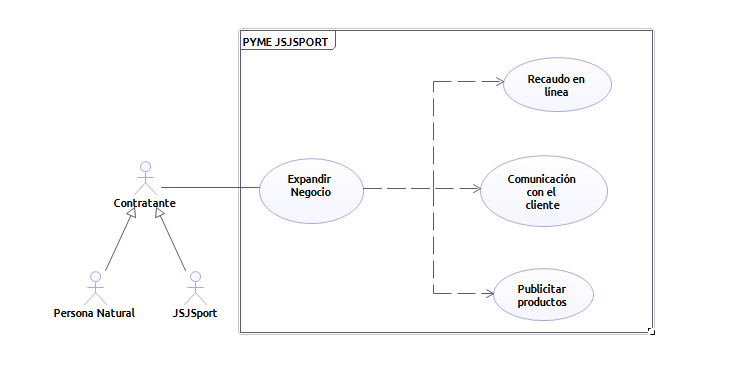
\includegraphics[width=0.7\linewidth]{arquitectura/imagenes/casosDeUso}
	\caption{Diagrama de  casos de Uso}
	\label{fig:casosUso}
\end{figure}

El proceso de expandir el negocio, como  se puede observar en la figura \ref{fig:casosUso}, incluye tres procesos importantes, el primero de ellos es que el sistema pueda publicitar productos, en otras palabras,  brindar al cliente una plataforma web donde pueda exponer sus productos hacia al público deseado, teniendo en cuenta los aspectos como su inventario, apoyándose con una base de datos.\newline
El proceso de comunicación con el cliente consiste en todo lo  relacionado al proceso de asesoría que se le brinda al cliente en la página, durante todo el proceso de compra que ese realice podrá consultar el cualquier momento a algún asesor cualquier duda o inquietud que le surja con respecto a los productos o a los procesos de pago. \newline
El proceso de recaudo en línea, consiste en todo lo relacionado con la compra y venta del producto que se ofrecen en la plataforma web anteriormente generada, y verifica que el medio de pago ingresado por el usuario sea válido, una vez se compruebe el paso anterior se procederá a la confirmación de la compra, generando un comprobante de pago para la empresa y para el usuario para finalmente  proceder a pedirle al usuario que ingrese los datos del domicilio.



\newpage


\section{Escenarios}
En este seccion observaremos el modelamiento desde los cimientos de nuestra plataforma, de la seccion anterior concluimos el "QUE" del sistema o dicho en otras palabras que es lo que el cliente desea, a partir de la toma y organización de requerimientos procedemos a hacer un análisis del sistema que vamos a diseñar, a continuación observaremos diferentes herramientas que nos proveen unas bases para empezar a realizar nuestro sistema, conoceremos información actual y propondremos a grandes rasgos un modelo de posible solución a nuestro problema. 


\subsection{Diagrama de secuencia}

Un diagrama de secuencia es una herramienta que proporciona al usuario y al desarrollador el “COMO” del sistema, esto se refiere a como se van a abordar los requerimientos obtenidos en nuestro primer capítulo, estos requerimientos, ahora llamados procesos deben ser abordados por los actores que interactuaran directamente con el sistema, y de esta manera  que debe el sistema responder para llevar a cabo el proceso de manera óptima.

En nuestro caso los procesos que abordaremos para dar respuesta a esta pregunta son los que mostraremos a continuación.

\begin{figure}[th!]
	\centering
	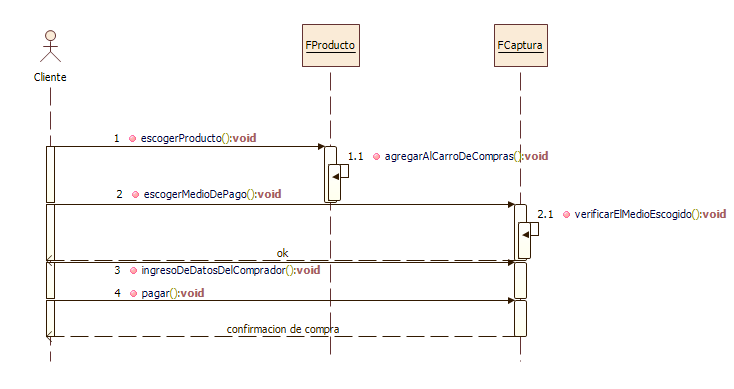
\includegraphics[width=1.0\linewidth]{arquitectura/imagenes/DiagramaDeSequenciaRE}
	\caption{Diagrama de secuencia Recaudo en Línea}
\end{figure}

En el diagrama de secuencia anterior, se describe la secuencia entre el cliente, un formulario de captura y un formulario de producto. Inicialmente el cliente escogerá un producto, lo que genera un llamado a formulario producto, quien a su vez, hace un llamado recursivo para agregar al carro de compras, terminado este proceso el cliente escogerá un medio de pago, haciendo un llamado al formulario de captura, quien antes de retornar un mensaje satisfactorio, verificara el medio de pago escogido y retornara un "ok", tras recibir el mensaje de satisfacción del medio de pago, el cliente ingresara sus datos en el formulario de captura y posteriormente seleccionara pagar, para lo cual recibirá una confirmación de compra.


\newpage
\begin{figure}[th!]
	\centering
	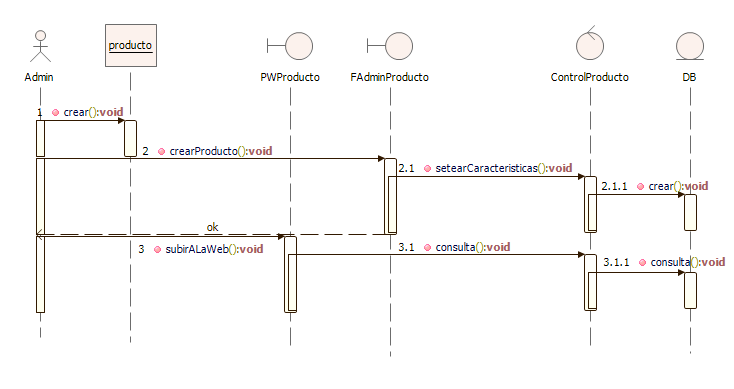
\includegraphics[width=1.0\linewidth]{arquitectura/imagenes/DiagramaDeSecuenciaPP}
	\caption{Diagrama de secuencia Publicitar Producto}
\end{figure}
En el diagrama de secuencia anterior, se describe el proceso para crear y publicar un producto en la plataforma web del cliente. Inicialmente el administrador (cliente) deberá crear el producto, posteriormente seleccionara crear el producto mediante un formulario de administrador, en el cual colocara (seteara) las características del mismo, las cuales pasaran por una clase de control de producto y este a su vez creara el producto en la base de datos, con lo cual el formulario de administración del producto, retornara un mensaje de satisfacción. Por último el administrador, seleccionara subir a la web, haciendo un llamado a la interfaz PW producto, quien hará una consulta del producto, por medio de la clase control producto, para hacer una consulta en la base de datos.

\begin{figure}[th!]
	\centering
	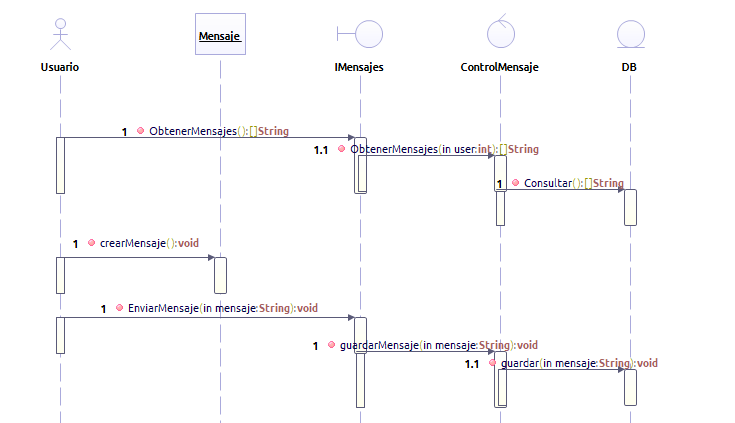
\includegraphics[width=1.0\linewidth]{arquitectura/imagenes/DiagramaDeSecuenciaCC}
	\caption{Diagrama de secuencia Comunicación con el cliente}
	\label{img:secuenciacomcliente}
\end{figure}

En la figura \ref{img:secuenciacomcliente} se puede observar el proceso que se realizara cuando un usuario independientemente de su rol (cliente/asesor) desee crear o establecer una comunicación con su contraparte, asesor->cliente y cliente->asesor. Inicialmente el usuario deberá ingresar al módulo de comunicación y allí se hará una consulta de todos los mensajes enviados y recibidos previamente y se mostrarán en estilo de conversación, posteriormente el usuario creara un mensaje redactando el contenido de este y lo enviara, este pasara por una interfaz de mensajes que accederá a la clase de control de mensajes y lo guardará en la base.

\subsection{Diagrama de comunicación}
Un diagrama de comunicación le sirve al desarrollador para modelar las interacciones entre los objetos que hacen parte de un sistema en términos de mensajes en secuencia, esto se refiere a todas las acciones que pueden realizar los objetos del sistema sobre otros objetos del mismo sistema, después de realizado un diagrama de secuencia se facilita la creación de los diagramas de comunicación.

A continuación mostraremos diagramas de comunicación de los procesos realizados en los anteriores diagramas de secuencia

\begin{figure}[h!]
	\centering
	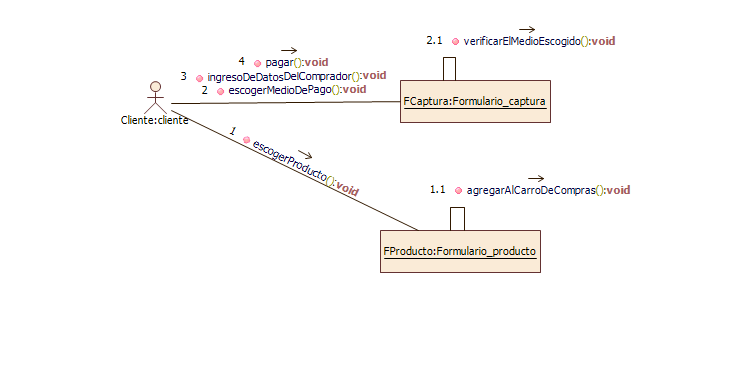
\includegraphics[width=1.1\linewidth]{arquitectura/imagenes/Diagrama_comunicacion_re}
	\caption{Diagrama de comunicación Recaudo en Línea}
\end{figure}

El diagrama de comunicación anterior, describe mediante que mensajes se comunica el cliente con las clases formulario de captura y formulario de producto. Con el formulario de captura se comunica mediante los mensajes, pagar, ingreso de datos del comprador, y escoger medio de pago, y con el formulario de producto se comunica mediante el mensaje  escoger producto, adicionalmente el formulario de captura se comunica, consigo mismo, mediante verificar medio de pago escogido, y el formulario de producto se comunica consigo mismo, mediante el mensaje agregar al carrito de compras.


\newpage
\begin{figure}[th!]
	\centering
	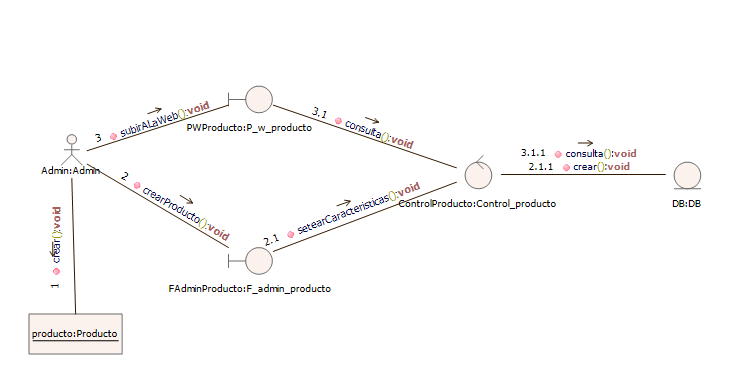
\includegraphics[width=1.1\linewidth]{arquitectura/imagenes/Diagrama_comunicacion_pp}
	\caption{Diagrama de comunicación Promocionar Productos}
	\label{fig:diagramacomunicacionpp}
\end{figure}

El diagrama de comunicación anterior, muestra la comunicación entre el cliente (administrador) y la interfaz PW producto (mediante el mensaje subir a la web) y la interfaz Formulario de administración producto, mediante el mensaje crear producto, quienes se comunican con la clase control producto, mediante los mensajes de consulta y setear características respectivamente, por otro lado, el administrador se comunica con el objeto producto, mediante el mensaje de creación. Por ultimo la clase control producto, se comunica con la base de datos, con los mensajes de consulta y creación de productos.

\begin{figure}[th!]
	\centering
	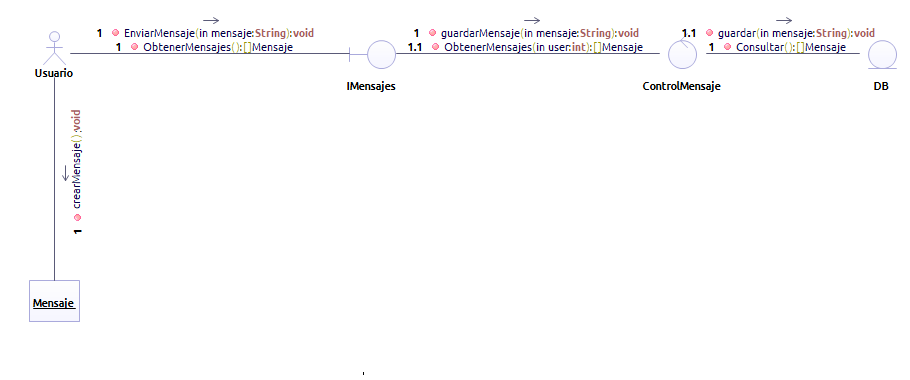
\includegraphics[width=1.1\linewidth]{arquitectura/imagenes/Diagrama_comunicacion_cc}
	\caption{Diagrama de comunicación para Gestión de Mensajes}
	\label{fig:diagramaComunicacionMensajes}
\end{figure}

Como se puede ver en la figura \ref{fig:diagramaComunicacionMensajes} la comunicación entre el usuario y la interfaz de mensajes se da cuando el cliente desea consultar sus mensajes o enviar un mensaje que escribió, la interfaz de mensajes a su vez se conecta con el control del mensaje el cual permite hacer las diferentes comunicaciones a la base de datos conforme al proceso que se necesite.
\newpage

\section{Clases}
Un diagrama de clases es una forma de visualización de código de programación llevado a un nivel más sencillo para que el desarrollador tenga un mayor nivel de comprensión, por medio de estos diagramas se evidencia que existen soluciones a problemas recurrentes, estos son llamados patrones, el uso de patrones en el desarrollo de software no solo optimiza el funcionamiento del sistema si no permite la escalabilidad y la agregación de nuevas funciones 

Para la solución propuesta al problema de la PYME JSJSports se presentan los siguientes diagramas de clases, usando patrones de diseño para el desarrollo de un sistema óptimo y escalable.

\newpage

\section{Componentes}
Un componente es un objeto dentro de un sistema que cumple una funcionalidad específica, en un diagrama de componentes se pueden observar varios componentes relacionados entre sí, los componentes cumplen la característica que son cajas negras y además pueden implementar interfaces entre ellos.

\begin{figure}[th!]
	\centering
	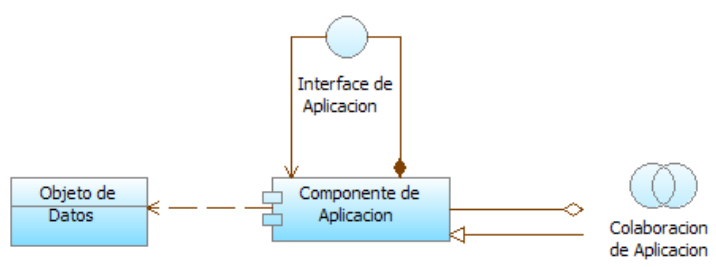
\includegraphics[width=0.7\linewidth]{arquitectura/imagenes/modeloEstructuraAplicacion}
	\caption{Metamodelo un Diagrama de Componentes}
	\label{fig:metamodeloComponentes}
\end{figure}

\subsection*{Caso de estudio}
\begin{figure}[th!]
	\centering
	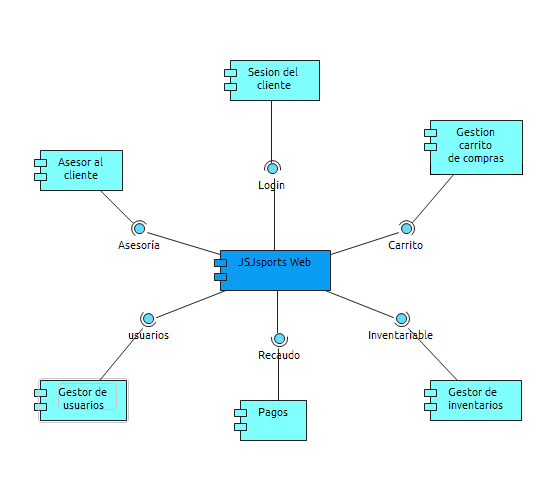
\includegraphics[width=0.7\linewidth]{arquitectura/imagenes/PuntoVistaEstructuraAplicacion}
	\caption{Diagrama de Componentes}
	\label{fig:componentes}
\end{figure}

En este diagrama de componentes podemos observar cada uno de los componentes del sistema y las interfaces que funcionan como pegamento para estos componentes con el con el componente  central JSJSport Web, la interfaz asesoría permite brindar asesoría al usuario y es la que se encarga de realizar todo los procesos de comunicación, la interfaz login le permite al usuario administrar su sesión e ingresar o salir del sistema, la interfaz carrito ayuda a manejar el carrito de compras y los productos que desea el usuario. La interfaz recaudo permite gestionar los pagos de las compras realizadas, la interfaz de usuarios permite gestionar los usuarios y sus roles y permisos, por último la interfaz inventariable permite hacer la gestión de los inventarios y productos que tiene la PYME.

\newpage

\section{Nodos}
Un diagrama de nodos nos permite como desarrolladores conocer los recursos físicos necesarios para que el sistema sea implementado, hay dos tipos de nodos, nodos dispositivo y procesador con los cuales tanto el desarrollador como el cliente puede interactuar, esto representa la comunicación y las relaciones entre el hardware para la modelación del sistema.

A continuación observaremos el diagrama de nodos para nuestra plataforma web:

\begin{figure}[h]
	\centering
	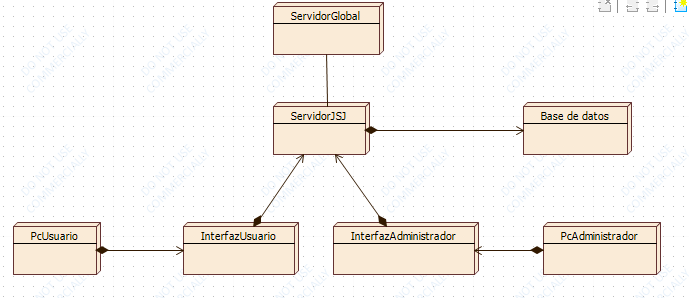
\includegraphics[width=0.7\linewidth]{arquitectura/imagenes/DiagramaNodos}
	\caption{Diagrama de nodos}
	\label{fig:diagramanodos}
\end{figure}

Como podemos observar en el caso de nuestro proyecto se observan 7 nodos de los cuales el nodo del servidor jsj, la base de datos, y las páginas de las interfaces de usuario y administrador son primordiales
En el nodo del servidor jsj se tienen todos los componentes que permiten el funcionamiento de la página de ventas de artículos deportivos
Entre estos componentes encontramos acciones que serán ejecutadas dependiendo del tipo de usuario que ingrese
Para el caso de la interfaz administrativa, contara con acciones como agregar, modificar o eliminar productos, estableciendo una conexión con los componentes del servidor que permiten realizar dichas acciones
En el caso de la interfaz de usuario se dispondrá de acciones como la compra de los productos, y todo el proceso que conllevando estableciendo una comunicación con el servidor jsj que llamara a dichos componentes
El servidor jsj tambien nececita una comunicación con una base de datos que se encargará de almacenar todo tipo de información relacionada con la pagina, como los productos, los usuarios, información de los pedidos, etc
Los otros nodos que podemos encontrar como pc de usuario y de admin son recursos fisicos necesarios para la comunicacion con la pagina web. \newline
En el punto de vista de uso de infraestructura en la figura \ref{modeloUsoInfraestructura} se puede observar de forma más clara lo que se encuentra en el nodo del servidor JSJ, y las interacciones con las interfaces del administrador y del cliente, dentro del servidor de JSJ encontramos cada uno de los componentes definidos para el sistema integrados en función de satisfacer cada una de las necesidades de los usuarios.
\newpage

\section{Sistemas}
También llamado diagrama de paquetes se observa la organización jerárquica y la relación que tienen los paquetes de los cuales se compone el sistema, a partir de este podemos observar el rendimiento del sistema por medio de la evaluación de métricas.

En el siguiente diagrama se evidencia la organización de cada una de las partes del proyecto y su ubicación en los diferentes paquetes que implementa el mismo, en este caso dentro de la aplicación web de JSJSports en el paquete de componentes encontramos todos los componentes definidos anteriormente dentro del paquete com. Además de los componentes encontramos el api y las utilidades que son los que nos permitirán hacer el pegamento con los componentes y cargar cada no de los mismos componentes necesarios para el funcionamiento.

En la parte inferior de la figura \ref{fig:sistemas} se puede observar el paquete com, en donde básicamente se encuentra la presentación que tiene todos los aspectos de la vista, el repositorio que se encarga de la persistencia y el paquete más importante el cableado que se encarga de realizar todo el cableado de la aplicación y estructurarla.



\begin{figure}[h!]
	\centering
	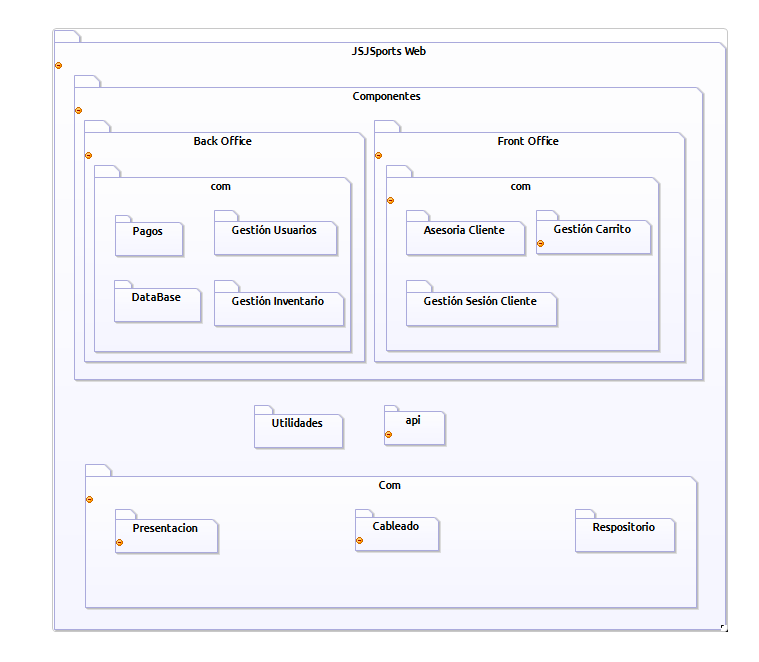
\includegraphics[width=0.9\linewidth]{arquitectura/imagenes/DiagramaDeSistemas}
	\caption{Diagrama de Sistemas}
	\label{fig:sistemas}
\end{figure}


\newpage

\section{Diagrama de Actividades}
Un diagrama de actividades permite al desarrollador observar cómo se está realizando el proceso y como se comunican los diferentes actores, dentro de dichas actividades puede haber decisiones pero siempre el proceso debe acabar.\newline
Muestra un proceso de negocio o un proceso de software como un lujo de trabajo a través de una serie de acciones. Las personas, los componentes de software o los equipos pueden realizar estas actividades.
Puede usar un diagrama de activiades para describir procesos de varios tipos, como los ejemplos siguientes:
\begin{itemize}
   \item Un proceso de negocio o un flujo de trabajo entre los usuarios y el sistema.
	\item Los pasos que se realizen en un caso de uso.
	\item Un protocolo de software, es decir, las secuencias de interacciones entre componentes permitidos.
	\item Un algoritmo de Software
\end{itemize} 

\subsection*{Caso de Estudio}

En el siguiente diagrama de actividades se muestra como es el proceso de la compra de un producto, en la que intervienen 3 actores principales:
\begin{enumerate}
	\item Comprador: Se encarga de escoger el producto, que desea comprar, seleccionando un método de pago y recibiendo la confirmación de compra del mismo.
	\item Plataforma: Se encarga de presentar el producto al comprador, y es el enlace entre en el comprador y el inventario, para la realización de cada acción.
	\item Inventario: Se encarga de verificar la disponibilidad de cada producto, y actualizar el inventario del mismo.
\end{enumerate}

\begin{figure}[th!]
	\centering
	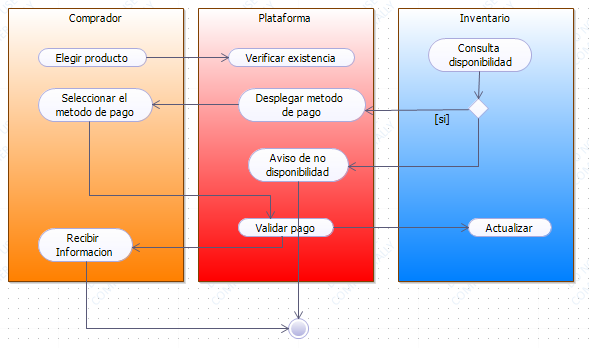
\includegraphics[width=1\linewidth]{arquitectura/imagenes/workflow}
	\caption{Diagrama de actividades para la compra de un producto}
	\label{fig:workflow}
\end{figure}


El proceso de compra de un producto empieza por el comprador que es el que escoge el producto deseado, enviando una petición a la plataforma, para verificar su existencia, la cual hace la consulta en el inventario para ver su disponibilidad, en este paso hay dos posibles opciones, en el caso de que no sea disponible, envía un aviso a la plataforma para que informe al comprador y se acaba la acción, en el caso de que sea disponible, la plataforma muestra los métodos de pago disponibles, una vez que el comprador escoja un método de pago, se validara en la plataforma y se procederá a enviar la facturación al comprador y a la actualización del inventario del producto.

\begin{figure}[th!]
	\centering
	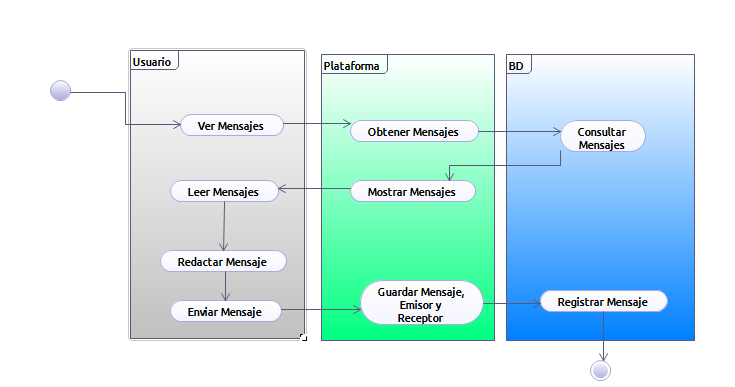
\includegraphics[width=1\linewidth]{arquitectura/imagenes/workflowMensajes}
	\caption{Diagrama de actividades para proceso de comunicación}
	\label{fig:workflowMensajes}
\end{figure}

En la figura \ref{fig:workflowMensajes} se puede observar las actividades implicadas en el proceso de comunicación de dos usuarios del sistema (asesor->cliente o cliente->asesor), para ver los mensajes es necesario que este se solicite ver los mensajes y la plataforma solicitara a la bd los mensajes del usuario y los mostrara, una vez el usuario lea los mensajes podrá redactar un mensaje y enviarlo, allí la plataforma solicitará a la base de datos registrar el respectivo mensaje.

\newpage

\section{Estados}
Los estados son aquellas fases en las que el sistema puede estar, un diagrama de estados permite observar como son las transiciones entre estas fases, y cuáles son los lanzadores que con una condición activan estas transiciones, los estados son únicos. 

A continuación veremos el diagrama de estados para el sistema de compra en línea planteado:

\begin{figure}[th!]
	\centering
	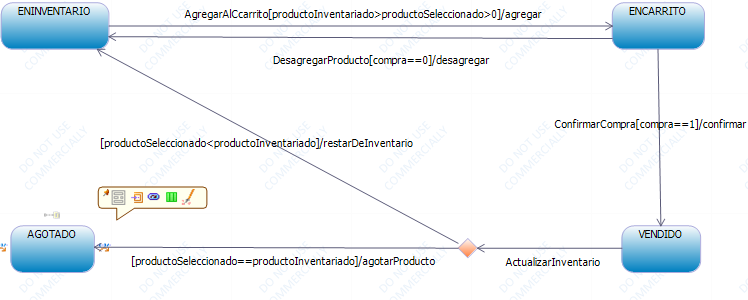
\includegraphics[width=0.9\linewidth]{arquitectura/imagenes/diagramas_estados}
	\caption{Diagrama de estado producto}
\end{figure}

En el anterior Diagrama de estados podemos ver la transición que tienen los productos desde el momento en que se cargan a la página, hasta que se realiza exitosamente una  compra, para esto nos basamos en 4 estados posibles, en inventario, en carrito, vendido, agotado, el producto empieza en un estado base de en inventario con una cantidad disponible, cuando se agrega el producto a carrito se cambia de estado a en carrito, en donde tiene dos posibles disparadores, que son desagregar de carrito y confirmar compra, si se desagrega del carrito, regresara a su estado base en inventario, si se confirma la compra cambiara de estado ha vendido, en donde se actualizara el inventario, si la cantidad comprada es igual a la disponibles en inventario, el producto quedara en un estado de agotado, si aún hay unidades disponibles volverá a un estado de inventario, a partir de ahí podemos crear una clase producto la cual podrá contener cualquiera de los 4 estados como se muestra a continuación:


\begin{figure}[th!]
	\centering
	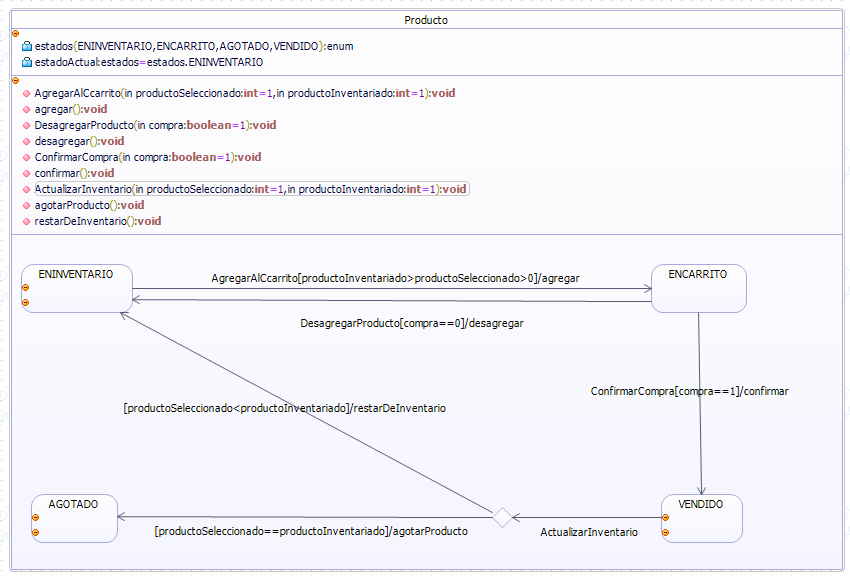
\includegraphics[width=0.7\linewidth]{arquitectura/imagenes/clase_producto_estados}
	\caption{Clase producto estado}
\end{figure}

En este diagrama de clase se muestran los métodos necesarios para realizar las transiciones de un estado.
\newpage






